% Provenance (never printed): see sources/outline_sources.md (Year 2: partial melting of the
% mantle; solidus and geotherm; decompression, hydration and heating; degree of melting;
% binary and ternary phase diagrams applied to rocks).
% Curves from figdata/bachelor-2/melting.py (Bowen 1915 diopside-anorthite, Bowen and
% Andersen 1914 forsterite-silica, Katz et al. 2003 melting of peridotite); exercise and
% problem values in the Book 4 scratch calculator calc/ch07.py.
\chapter{انصهار الوشاح}\label{ch:b2:mantle-melting}

الوشاح صلب. فالموجات الزلزالية القصّية تعبره من أعلاه إلى أسفله،
\omterm{def:b2:mantle-melting:peridotites}{والبيريدوتيت} الذي يُجلب منه صخر بلّوري. ومع ذلك فهو يعطي على امتداد الظهرات
المحيطية وحدها نحو عشرين كيلومترًا مكعبًا من القشرة المحيطية الجديدة كل سنة،
وكل متر مكعب منها مصنوع من مصهور. ويزول هذا التناقض حين نعرف
أن الوشاح لا ينصهر لأنه يُسخَّن: بل ينصهر لأن الضغط
عليه ينخفض، أو لأن الماء يُضاف إليه. فتحت الظهرة يصعد
الوشاح، وينخفض ضغطه أسرع من درجة حرارته، فيعبر
منحنى انصهاره؛ وفوق لوح هابط، يخفض الماء المتحرّر من اللوح ذلك
المنحنى تحت إسفين الوشاح. وفي الحالتين لا ينصهر إلا كسر صغير من الصخر،
وهذا الكسر، حين ينفصل عن بقاياه، يصير بازلت
قاع المحيط والأقواس البركانية. يصف هذا الفصل أولًا صخر الوشاح
ومخطّطات الأطوار التي تبيّن كيف تنصهر مثل هذه الصخور، ثم يتتبّع
الوشاح صاعدًا تحت ظهرة حتى سمك القشرة التي يصنعها.
% ledger: white:crust (Book 3), data:pb2002 (Book 3), katz03:solidus

\begin{recall}
\textbf{من مجلد السنة الثانية من كتب الكيمياء}: مخطّطات الأطوار الثنائية،
وخط الصلابة وخط السيولة، ونقطة الأوتكتيك، والانصهار المتطابق، والمحاليل الصلبة
وقاعدة الرافعة، التي تتناسب بموجبها نسبتا طورين متعايشين
تناسبًا عكسيًا مع بعديهما عن التركيب الكلي.
\textbf{من كتب الفيزياء}: السعة الحرارية النوعية، والحرارة الكامنة، والإنتروبيا
والمبدأ الثاني، الذي تحفظ بموجبه العملية الكظومة العكوسة الإنتروبيا.
\textbf{من مجلد السنة الأولى}: المعادن الرئيسية المكوّنة للصخور، الأوليفين
والبيروكسينات والغارنت والسبينل، ومحاليلها الصلبة ورقم المغنيسيوم؛
والتدرّج الكظوم للوشاح، $\mathrm dT/\mathrm dz = \alpha gT/c_p$؛ والقشرة المحيطية،
التي يبلغ سمكها \qty[uncertainty-mode=separate]{7.1 \pm 0.8}{km} بعيدًا عن النقاط الساخنة
ونحو \qty{20}{km} فوق لبّ عمود وشاحي؛ والألواح المندسّة والماء الذي
تحمله. \textbf{من \cref{ch:b2:elements-in-the-earth}}: \omterm{def:b2:elements-in-the-earth:morb-oib}{بازلت الظهرات وسط المحيطية}
(MORB)، ومعاملات التوزيع والعناصر غير المتوافقة.
\end{recall}

\section{صخر الوشاح}\label{sec:b2:mantle-melting:rock}

يبلغ صخر الوشاح السطح قطعًا تحملها الصهارات إلى الأعلى، هي
الصخور الدخيلة (الزينوليثات)، وقاعدةً لشرائح من الغلاف الصخري المحيطي دُفعت فوق
القارات، هي الأفيوليتات. وكلّه تقريبًا بيريدوتيت.
% ledger: geo:peridotite (Book 2), tulane:ocean-basins (Book 2)

\begin{definition}[البيريدوتيت وأنواعه]\label{def:b2:mantle-melting:peridotites}
\emph{البيريدوتيت}\index{البيريدوتيت} صخر فوق مافي خشن الحبيبات
يحوي أكثر من \qty{40}{\percent} من الأوليفين، والباقي بيروكسينات
وقليل من معدن ألومينيومي (سبينل أو غارنت).
و\emph{الدونيت}\index{الدونيت} يحوي أكثر من \qty{90}{\percent} من الأوليفين. وتحت
ذلك، يحوي \emph{اللرزوليت}\index{اللرزوليت} الأورثوبيروكسين
والكلينوبيروكسين كليهما؛ ويحوي \emph{الهارزبورجيت}\index{الهارزبورجيت} الأورثوبيروكسين لكن
لا يكاد يحوي كلينوبيروكسين؛ ويحوي الويرليت الكلينوبيروكسين لكن لا يكاد يحوي
أورثوبيروكسين. والصخور التي فيها أقل من \qty{40}{\percent} من الأوليفين بيروكسينيتات.
\end{definition}
% ledger: bgs:ultramafic

يُقرأ التصنيف على مثلث رؤوسه الأوليفين
والأورثوبيروكسين والكلينوبيروكسين (الشكل أدناه): كل نقطة تمثّل صخرًا،
وأبعادها عن الأضلاع الثلاثة تعطي نسب المعادن
الثلاثة. ولتركيب نموذجي للوشاح العلوي المستنزَف الذي ينصهر تحت
الظهرات \qty{57}{\percent} من الأوليفين،
و\qty{28}{\percent} من الأورثوبيروكسين، و\qty{13}{\percent} من الكلينوبيروكسين
و\qty{2}{\percent} من السبينل: إنه لرزوليت.
% ledger: liang21:dmm-mode

\begin{omfigure}
\centering
\begin{tikzpicture}[x=1.25cm, y=1.25cm, font=\scriptsize]
\coordinate (O) at (2.5,4.330); \coordinate (P) at (0,0); \coordinate (C) at (5,0);
\fill[green!8] (2.25,3.897) -- (2.75,3.897) -- (O) -- cycle;
\fill[orange!10] (1,1.732) -- (2.25,3.897) -- (2.75,3.897) -- (4,1.732) -- cycle;
\draw[thick] (O) -- (P) -- (C) -- cycle;
\draw (2.25,3.897) -- (2.75,3.897);
\draw (1,1.732) -- (4,1.732);
\draw (2.5,3.897) -- (1.25,1.732);
\draw (2.5,3.897) -- (3.75,1.732);
\node[anchor=south] at (O) {أوليفين};
\node[anchor=north east] at (P) {أورثوبيروكسين};
\node[anchor=north west] at (C) {كلينوبيروكسين};
\node[anchor=west] at (2.85,4.05) {دونيت};
\draw (2.5,4.05) -- (2.8,4.05);
\node at (2.5,2.05) {لرزوليت};
\draw (1.85,3.0) -- (0.75,3.3) node[anchor=east] {هارزبورجيت};
\draw (3.15,3.0) -- (4.25,3.3) node[anchor=west] {ويرليت};
\node at (2.5,0.85) {بيروكسينيتات};
\node[anchor=east] at (0.95,1.732) {\foreignlanguage{arabic}{أوليفين بنسبة \qty{40}{\percent}}};
\node[anchor=east] at (2.2,3.897) {\qty{90}{\percent}};
\fill[red!70!black] (2.12,2.52) circle (2pt);
\draw[red!70!black] (2.12,2.52) -- (4.4,2.52) node[anchor=west] {نموذج الوشاح};
\end{tikzpicture}
\par\smallskip{\small تصنيف البيريدوتيتات والبيروكسينيتات حسب
نسب الأوليفين والأورثوبيروكسين والكلينوبيروكسين فيها (عن مخطّط هيئة المسح
الجيولوجي البريطانية). والشريطان الضيّقان على امتداد الضلعين العلويين يضمّان
الصخور التي لا تكاد تحوي كلينوبيروكسين (\omterm{def:b2:mantle-melting:peridotites}{الهارزبورجيت}) أو لا تحوي أورثوبيروكسين (الويرليت).
والنقطة الحمراء هي نموذج الوشاح العلوي تحت الظهرات (57 و28
و\qty{13}{\percent}، بعد إعادة التطبيع دون ما فيه من السبينل، \qty{2}{\percent}).}
\end{omfigure}
% ledger: bgs:ultramafic, liang21:dmm-mode

البيريدوتيتات الثلاثة ليست ثلاثة أنماط صخرية مستقلة: إنها مراحل
عملية واحدة. فالكلينوبيروكسين والمعدن الألومينيومي يُستنفدان أولًا حين
ينصهر \omterm{def:b2:mantle-melting:peridotites}{البيريدوتيت} (\cref{sec:b2:mantle-melting:decompression})، \omterm{def:b2:mantle-melting:peridotites}{فاللرزوليت}
الذي فقد مصهورًا يصير أفقر بهما؛ وبعد انصهار كافٍ يصير
هارزبورجيتًا، والصخر الذي فقد كل بيروكسينه تقريبًا دونيت.
% ledger: katz03:melting

\begin{definition}[الوشاح الخصب والوشاح المتبقّي]\label{def:b2:mantle-melting:fertility}
\emph{الوشاح الخصب}\index{الوشاح الخصب} بيريدوتيت، لرزوليت عادة،
لا يزال يحوي الكلينوبيروكسين والمعدن الألومينيومي اللذين
يُصنع منهما البازلت. و\emph{الوشاح المتبقّي}\index{الوشاح المتبقّي} هو
\omterm{def:b2:mantle-melting:peridotites}{البيريدوتيت} الباقي بعد أن استُخلص منه مصهور: أفقر في
الكلينوبيروكسين والألومنيوم والكالسيوم والعناصر غير المتوافقة، وأغنى في
الأوليفين وذو رقم مغنيسيوم أعلى.
\end{definition}

\omterm{def:b2:isotope-geochemistry:reservoirs}{الوشاح المستنزَف} النظائري في \cref{ch:b2:isotope-geochemistry} خزّان،
يُعرَّف بنسبه؛ أمّا \omterm{def:b2:mantle-melting:fertility}{الوشاح المتبقّي} فصخر، يُعرَّف بما فقده.
والاثنان مرتبطان، لأن \omterm{def:b2:isotope-geochemistry:reservoirs}{الوشاح المستنزَف} مستنزَف لأن مصهورًا
استُخلص منه منذ زمن بعيد، لكن أحدهما يُقرأ في مطياف الكتلة والآخر
تحت المجهر.

\section{مخطّطات أطوار الصخور}\label{sec:b2:mantle-melting:diagrams}

الصخر خليط من المعادن، وهو ينصهر على مدى من درجات الحرارة، لا عند
نقطة واحدة. وقد قيست المخطّطات التي تصف ذلك أولًا على خلائط من
معادن صناعية نقية، بإبقاء شحنة صغيرة عند درجة حرارة معلومة حتى
تبلغ التوازن، ثم سقيها بسرعة، والبحث تحت المجهر عن الزجاج،
الذي كان سائلًا، وعن البلّورات.

\subsection*{أوتكتيك ثنائي: الديوبسيد والأنورثيت}

يتكوّن البازلت أساسًا من بلاجيوكلاز كلسي وكلينوبيروكسين،
وقد اختار بوين الأنورثيت والديوبسيد النقيين نموذجًا أبسط له. فإذا خُلطا وسُخّنا،
كوّنا نظامًا أوتكتيكيًا
عاديًا (الشكل أدناه): ينصهر الديوبسيد عند \qty{1391.5}{\celsius} والأنورثيت
عند \qty{1550}{\celsius}، لكن خليطًا من \qty{58}{\percent} من الديوبسيد
و\qty{42}{\percent} من الأنورثيت كتلةً ينصهر كليًا عند \qty{1270}{\celsius}.
% ledger: bowen15:di-an

\begin{omfigure}
\centering
\begin{tikzpicture}
\begin{axis}[omrecord, width=0.78\linewidth, height=6cm,
  xmin=0, xmax=100, ymin=1200, ymax=1600,
  xlabel={\foreignlanguage{arabic}{الأنورثيت \babelsublr{(\unit{\percent})} كتلةً}}, ylabel={\foreignlanguage{arabic}{درجة الحرارة \babelsublr{(\unit{\celsius})}}},
  y tick label style={/pgf/number format/1000 sep={}},
  tick label style={font=\scriptsize}, label style={font=\small}]
\addplot[very thick, black] table[x=x_an, y=T] {figdata/out/bachelor-2-melting-di-an-liq.dat};
\addplot[only marks, mark=*, mark size=1.6pt, blue!70!black] table[x=x_an, y=T] {figdata/out/bachelor-2-melting-di-an-data.dat};
\draw[thick] (axis cs:0,1270) -- (axis cs:100,1270);
\draw[densely dotted, red!70!black, thick] (axis cs:20,1590) -- (axis cs:20,1270);
\draw[->, red!70!black, thick] (axis cs:20,1350) -- (axis cs:41,1272);
\fill[red!70!black] (axis cs:20,1350) circle (1.6pt);
\node[font=\scriptsize] at (axis cs:55,1500) {سائل};
\node[font=\scriptsize, align=center] at (axis cs:10,1300) {ديوبسيد\\+ سائل};
\node[font=\scriptsize, align=center] at (axis cs:72,1360) {أنورثيت + سائل};
\node[font=\scriptsize] at (axis cs:68,1235) {ديوبسيد + أنورثيت};
\node[font=\scriptsize, anchor=north east] at (axis cs:41,1267) {\foreignlanguage{arabic}{النقطة E، \qty{1270}{\celsius}}};
\node[font=\scriptsize, anchor=west, red!70!black] at (axis cs:21,1360) {أول ديوبسيد};
\end{axis}
\end{tikzpicture}
\par\smallskip{\small النظام ديوبسيد--أنورثيت عند الضغط الجوي، من
تجارب السقي لبوين (1915): درجات حرارة خط السيولة (النقاط، منتصفات
مجالات السقي) والأوتكتيك E. وبالأحمر، تبريد سائل فيه
\qty{20}{\percent} من الأنورثيت: يتبلور الديوبسيد ابتداءً من \qty{1350}{\celsius}،
وينزل السائل على خط السيولة حتى E، ويتبلور الباقي هناك خليطًا من
المعدنين كليهما.}
\end{omfigure}
% ledger: bowen15:di-an

إذا قُرئ المخطّط من أعلى، أخبر بترتيب التبلور. فسائل فيه
\qty{20}{\percent} من الأنورثيت يبدأ بتبلور الديوبسيد عند
\qty{1350}{\celsius}؛ والسائل، إذ يفقد الديوبسيد، يغتني بالأنورثيت
وينزل على خط السيولة حتى يبلغ الأوتكتيك، حيث ينضمّ الأنورثيت إلى
الديوبسيد وتبقى درجة الحرارة عند \qty{1270}{\celsius} حتى ينفد السائل
كله. وإذا قُرئ من أسفل، أخبر كيف ينصهر الصخر: أيًّا كانت نسبتا
المعدنين، يظهر أول سائل عند \qty{1270}{\celsius} وله
التركيب الأوتكتيكي. وهذا هو الدرس الأول للوشاح. فأول مصهور من
صخر ليس له تركيب الصخر: بل له التركيب الذي تحدّده
المعادن التي ينصهر منها، ويظهر عند درجة حرارة أدنى بكثير من درجات
انصهارها كلها.

\subsection*{الانصهار غير المتطابق: الفورستريت والسيليكا}

بعض المعادن لا تنصهر إلى سائل له تركيبها.

\begin{definition}[الانصهار غير المتطابق، النقطة البيريتكتيكية]\label{def:b2:mantle-melting:peritectic}
يُظهر المعدن \emph{انصهارًا غير متطابق}\index{الانصهار غير المتطابق} حين يتفكّك،
عند تسخينه، إلى جسم صلب آخر وسائل مختلف
التركيب، بدلًا من أن ينصهر إلى سائل له تركيبه. وعلى مخطّط
أطوار ثنائي، النقطة التي يتعايش فيها هذا السائل مع الجسمين الصلبين هي
\emph{نقطة بيريتكتيكية}\index{النقطة البيريتكتيكية}: وهي، خلافًا للأوتكتيك، لا تقع
بين تركيبي الجسمين الصلبين.
\end{definition}

الإنستاتيت، وهو الأورثوبيروكسين المغنيسي \ce{MgSiO3}، ينصهر \omterm{def:b2:mantle-melting:peritectic}{انصهارًا غير متطابق}. فعند
الضغط الجوي يتفكّك عند \qty{1557}{\celsius} إلى فورستريت،
\ce{Mg2SiO4}، وسائل أغنى قليلًا منه بالسيليكا؛ ولا تذوب كل
الفورستريت إلا عند \qty{1577}{\celsius} (الشكل أدناه). وقد وجد بوين
وأندرسن عام 1914 أن التفكّك يعطي \qty{5.5}{\percent} من
الفورستريت و\qty{94.5}{\percent} من السائل، كما تتنبّأ قاعدة الرافعة من
التراكيب الثلاثة (\cref{exo:b2:mantle-melting:6}). وأبعد نحو السيليكا، ينصهر الإنستاتيت
والكريستوباليت معًا عند أوتكتيك، \qty{1543}{\celsius}.
% ledger: bowen14:mgo-sio2

\begin{omfigure}
\centering
\begin{tikzpicture}
\begin{axis}[omrecord, width=0.78\linewidth, height=6cm,
  xmin=40, xmax=66, ymin=1450, ymax=1950,
  xlabel={\foreignlanguage{arabic}{نسبة \ce{SiO2} الكتلية \babelsublr{(\unit{\percent})}}}, ylabel={\foreignlanguage{arabic}{درجة الحرارة \babelsublr{(\unit{\celsius})}}},
  y tick label style={/pgf/number format/1000 sep={}},
  tick label style={font=\scriptsize}, label style={font=\small}]
\addplot[very thick, black] table[x=x_sio2, y=T] {figdata/out/bachelor-2-melting-fo-sio2-liq.dat};
\addplot[very thick, black, dashed] table[x=x_sio2, y=T] {figdata/out/bachelor-2-melting-fo-sio2-fo.dat};
\draw[thick] (axis cs:42.71,1450) -- (axis cs:42.71,1890);
\draw[thick] (axis cs:42.71,1557) -- (axis cs:60.86,1557);
\draw[thick] (axis cs:59.85,1450) -- (axis cs:59.85,1557);
\draw[thick] (axis cs:59.85,1543) -- (axis cs:66,1543);
\fill (axis cs:60.86,1557) circle (1.6pt);
\fill (axis cs:64.87,1543) circle (1.6pt);
\fill (axis cs:42.71,1890) circle (1.6pt);
\node[font=\scriptsize, anchor=south west] at (axis cs:42.9,1890) {\foreignlanguage{arabic}{انصهار الفورستريت، \qty{1890}{\celsius}}};
\node[font=\scriptsize] at (axis cs:56,1800) {سائل};
\node[font=\scriptsize] at (axis cs:48,1680) {فورستريت + سائل};
\node[font=\scriptsize] at (axis cs:51,1500) {فورستريت + إنستاتيت};
\node[font=\scriptsize, align=center] at (axis cs:63,1495) {إنستاتيت +\\كريستوباليت};
\node[font=\scriptsize, anchor=south] at (axis cs:61.3,1560) {P};
\node[font=\scriptsize, anchor=south] at (axis cs:64.87,1546) {E};
\node[font=\scriptsize, anchor=north, rotate=90] at (axis cs:42.71,1650) {\ce{Mg2SiO4}};
\node[font=\scriptsize, anchor=south, rotate=90] at (axis cs:59.85,1510) {\ce{MgSiO3}};
\end{axis}
\end{tikzpicture}
\par\smallskip{\small جزء من النظام \ce{MgO}--\ce{SiO2} عند الضغط
الجوي، عن بوين وأندرسن (1914). ينصهر الإنستاتيت (\ce{MgSiO3}) \omterm{def:b2:mantle-melting:peritectic}{انصهارًا
غير متطابق} عند \omterm{def:b2:mantle-melting:peritectic}{النقطة البيريتكتيكية} P، \qty{1557}{\celsius}، إلى فورستريت
وسائل فيه \qty{60.9}{\percent} من \ce{SiO2}؛ وE هي أوتكتيك الإنستاتيت--الكريستوباليت،
\qty{1543}{\celsius}. ولم يُقس خط سيولة الفورستريت إلا قرب
الإنستاتيت: والجزء المتقطّع مرسوم مستقيمًا حتى نقطة انصهار الفورستريت.}
\end{omfigure}
% ledger: bowen14:mgo-sio2

\omterm{def:b2:mantle-melting:peritectic}{النقطة البيريتكتيكية} هي الدرس الثاني للوشاح. فحين ينصهر \omterm{def:b2:mantle-melting:peridotites}{البيريدوتيت} لا
يذوب أورثوبيروكسينه ببساطة: بل يعطي الأوليفين للبقايا والسيليكا
للمصهور. فيكون المصهور إذن أغنى بالسيليكا من البيروكسينات،
والبقايا أغنى بالأوليفين من الصخر: وهذا هو المسار من \omterm{def:b2:mantle-melting:peridotites}{اللرزوليت} إلى \omterm{def:b2:mantle-melting:peridotites}{الهارزبورجيت}
\omterm{def:b2:mantle-melting:peridotites}{والدونيت}.

\subsection*{ثلاثة مكوّنات: المخطّط الثلاثي}

للصخور الحقيقية أكثر من معدنين. ومع ثلاثة، يحتاج التركيب إلى
مثلث، وتصير درجة الحرارة بعدًا ثالثًا.

\begin{definition}[مخطّط الأطوار الثلاثي، الخط المتبلور المشترك، الأوتكتيك الثلاثي]\label{def:b2:mantle-melting:ternary}
\emph{مخطّط الأطوار الثلاثي}\index{مخطّط الأطوار الثلاثي} يمثّل
توازنات نظام من ثلاثة مكوّنات عند ضغط معطى: كل نقطة من
المثلث تمثّل تركيبًا، والرؤوس المكوّنات النقية،
ويُرسم سطح السيولة خطوطَ تساوي حرارة أو حقولًا للمعادن
التي تتبلور أولًا. و\emph{الخط المتبلور المشترك}\index{الخط المتبلور المشترك} هو
الخط الذي يكون السائل على امتداده مشبعًا بمعدنين معًا فيبلورهما
كليهما وهو يبرد. وتنحدر الخطوط المتبلورة المشتركة من الأوتكتيكات الثنائية
على أضلاع المثلث وتلتقي عند \emph{الأوتكتيك
الثلاثي}\index{الأوتكتيك الثلاثي}، وهو أدنى درجة حرارة يوجد عندها سائل،
حيث تتبلور المعادن الثلاثة معًا.
\end{definition}

\begin{method}[قراءة مسار تبلور على مخطّط ثلاثي]\label{met:b2:mantle-melting:ternary}
حدّد موقع التركيب الكلي $X$ في المثلث والحقل الذي يقع فيه:
فمعدن ذلك الحقل يتبلور أولًا. وما دام ذلك المعدن وحده يتبلور،
يتحرك السائل في خط مستقيم مبتعدًا مباشرة عن رأس المعدن،
مرورًا بالنقطة $X$، لأن إزالة مكوّن نقي لا تغيّر إلا نسبته؛ وبقاعدة
الرافعة يكون الكسر الكتلي للبلّورات هو المسافة من $X$ إلى السائل
مقسومةً على المسافة من الرأس إلى السائل. وحين يبلغ السائل
خطًا متبلورًا مشتركًا، ينضمّ المعدن الثاني ويتبع السائل \omterm{def:b2:mantle-melting:ternary}{الخط المتبلور المشترك}
نزولًا حتى \omterm{def:b2:mantle-melting:ternary}{الأوتكتيك الثلاثي}، حيث يتبلور آخر السائل. والمكوّن
الذي لا يدخل في أيٍّ من البلّورات يبقى في السائل، فيعطي تركيزه
كسر السائل الباقي: $f_{\text{السائل}} = c_X/c_{\text{السائل}}$.
\end{method}

\begin{omfigure}
\centering
\begin{tikzpicture}[x=1cm, y=1cm, font=\scriptsize]
\coordinate (A) at (3,5.196); \coordinate (B) at (0,0); \coordinate (C) at (6,0);
\coordinate (eAB) at (1.2,2.078); \coordinate (eAC) at (4.65,2.338);
\coordinate (eBC) at (3.9,0); \coordinate (E) at (3.45,1.299);
\coordinate (X) at (3.0,3.118); \coordinate (L) at (3.0,1.455);
\fill[green!8] (A) -- (eAB) -- (E) -- (eAC) -- cycle;
\fill[orange!10] (B) -- (eAB) -- (E) -- (eBC) -- cycle;
\fill[blue!7] (C) -- (eAC) -- (E) -- (eBC) -- cycle;
\draw[thick] (A) -- (B) -- (C) -- cycle;
\draw[very thick, -{Stealth[length=4pt]}] (eAB) -- ($(eAB)!0.55!(E)$);
\draw[very thick] ($(eAB)!0.5!(E)$) -- (E);
\draw[very thick, -{Stealth[length=4pt]}] (eAC) -- ($(eAC)!0.55!(E)$);
\draw[very thick] ($(eAC)!0.5!(E)$) -- (E);
\draw[very thick, -{Stealth[length=4pt]}] (eBC) -- ($(eBC)!0.55!(E)$);
\draw[very thick] ($(eBC)!0.5!(E)$) -- (E);
\draw[red!70!black, thick, dashed] (A) -- (X);
\draw[red!70!black, very thick, -{Stealth[length=4pt]}] (X) -- (L);
\draw[red!70!black, very thick, -{Stealth[length=4pt]}] (L) -- ($(L)!0.85!(E)$);
\fill[red!70!black] (X) circle (2pt); \fill[red!70!black] (L) circle (1.6pt);
\fill (E) circle (2pt);
\node[anchor=south] at (A) {A}; \node[anchor=north east] at (B) {B};
\node[anchor=north west] at (C) {C};
\node[anchor=west, red!70!black] at (3.1,3.2) {$X$};
\node[anchor=north east, red!70!black] at (2.95,1.42) {$L_1$};
\node[anchor=north west] at (3.5,1.25) {E};
\node[anchor=east] at (eAB) {$e_{AB}$}; \node[anchor=west] at (eAC) {$e_{AC}$};
\node[anchor=north] at (eBC) {$e_{BC}$};
\node at (2.35,2.75) {\foreignlanguage{arabic}{حقل A}}; \node at (1.55,0.7) {\foreignlanguage{arabic}{حقل B}}; \node at (4.9,0.7) {\foreignlanguage{arabic}{حقل C}};
\end{tikzpicture}
\par\smallskip{\small نظام أوتكتيكي ثلاثي (تخطيطي). كل حقل يضمّ
السوائل التي يتبلور منها معدنه أولًا؛ والخطوط المتبلورة المشتركة (الأسهم
نحو انخفاض درجة الحرارة) تمتدّ من الأوتكتيكات الثنائية $e$ إلى \omterm{def:b2:mantle-melting:ternary}{الأوتكتيك الثلاثي}
E. والسائل $X$ في حقل A يبلور A، ويبتعد عن الرأس A
حتى يلاقي \omterm{def:b2:mantle-melting:ternary}{الخط المتبلور المشترك} A--B عند $L_1$؛ ثم يتبلور A وB
معًا نزولًا حتى E، حيث ينضمّ C إليهما (\cref{exo:b2:mantle-melting:11}).}
\end{omfigure}

وتُقرأ أنظمة المعادن الثلاثة المكوّنة للصخور على النحو نفسه. أمّا القواعد التي تحدّد عدد الأطوار التي يمكن أن تتعايش،
وسطوح الطاقة الحرة التي تُحسب منها مثل هذه المخطّطات، فموضعها
مجلد السنة الثالثة من هذه السلسلة.

\section{خط الصلابة والتدرّج الكظوم وثلاث طرق للانصهار}\label{sec:b2:mantle-melting:solidus}

لبيريدوتيت الوشاح خط صلابة، هو درجة الحرارة التي يظهر عندها أول مصهور منه،
وخط سيولة أعلى منه بكثير. وكلاهما يرتفع مع الضغط. وتعطي التجارب على
البيريدوتيتات الطبيعية، التي جمعها وضبطها كاتز وشبيغلمان ولانغموير عام 2003،
لخط الصلابة الجاف
\[
  T_{\mathrm{s}}(P) = 1085.7 + 132.9\,P - 5.1\,P^2
\]
(بالدرجات المئوية، و$P$ بالغيغاباسكال): \qty{1086}{\celsius} عند السطح،
و\qty{1331}{\celsius} عند \qty{2}{GPa}. وعند الأعماق نفسها يكون الوشاح أسخن أو
أبرد من ذلك حسب موضعه، ولمقارنة الأوشحة يُزال
أثر العمق.
% ledger: katz03:solidus

\begin{definition}[درجة الحرارة الكامنة للوشاح]\label{def:b2:mantle-melting:tp}
\emph{درجة الحرارة الكامنة للوشاح}\index{درجة الحرارة الكامنة للوشاح} $T_p$
هي درجة الحرارة التي تكون لكتلة من الوشاح الحملي لو
رُفعت إلى السطح على امتداد التدرّج الكظوم للوشاح، دون تبادل حرارة
ودون انصهار.
\end{definition}

على امتداد التدرّج الكظوم $\mathrm dT/\mathrm dP = \alpha T/(\rho c_p)$، وهو صيغة
التدرّج $\alpha gT/c_p$ المذكور أعلاه بدلالة الضغط، لأن $\mathrm dP = \rho
g\,\mathrm dz$. ومع $\alpha = \qty{4e-5}{K^{-1}}$ و$\rho = \qty{3300}{kg/m^3}$
و$c_p = \qty{1000}{J/(kg.K)}$، يبلغ نحو \qty{20}{K} لكل غيغاباسكال،
والغيغاباسكال الواحد يقابل \qty{30.9}{km} من الوشاح (\cref{exo:b2:mantle-melting:3}). وقد أعطى مجلد السنة الأولى
الوشاح درجة حرارة كامنة تقارب \qty{1350}{\celsius} من فيزياء
المعادن؛ وتتراوح التقديرات الصخرية للوشاح تحت الظهرات من 1280 إلى
\qty{1400}{\celsius}.
% ledger: katz03:thermo, katsura:adiabat (Book 3), herzberg:tp (Book 3)

\begin{proposition}[بدء الانصهار بتخفيف الضغط]\label{prop:b2:mantle-melting:onset}
الوشاح الذي درجة حرارته الكامنة $T_p$ ويصعد على امتداد التدرّج الكظوم $T = T_p + GP$ (حيث $G$
ثابت) يبدأ بالانصهار عند الضغط $P_0$ الذي يلاقي فيه التدرّجُ الكظوم
خطَّ الصلابة $T_{\mathrm s}(P) = a_1 + a_2P + a_3P^2$، وهو الجذر الأصغر للمعادلة
\[
  -a_3P^2 + (G - a_2)P + (T_p - a_1) = 0 .
\]
والوشاح الأسخن بمقدار $\Delta T_p$ يبدأ بالانصهار على عمق أكبر، بمقدار $\Delta P_0 \approx
\Delta T_p/(T_{\mathrm s}'(P_0) - G)$.
\end{proposition}

\begin{proof}
في العمق يكون التدرّج الكظوم أبرد من خط الصلابة، لأن خط الصلابة يرتفع
أشدّ انحدارًا ($T_{\mathrm
s}' \approx \qty{110}{K/GPa}$ مقابل $G \approx 20$). ويتقاطع المنحنيان حيث
$T_p + GP = a_1 + a_2P + a_3P^2$، وهي تؤول بإعادة الترتيب إلى المعادلة التربيعية. واشتقاق
$T_p + GP_0 = T_{\mathrm s}(P_0)$ يعطي $\mathrm dT_p = (T_{\mathrm s}'(P_0) -
G)\,\mathrm dP_0$.
\end{proof}

من أجل $T_p = \qty{1350}{\celsius}$ يكون البدء عند \qty{2.66}{GPa}، أي على عمق نحو
\qty{82}{km}، عند \qty{1403}{\celsius}؛ وكل \qty{10}{\celsius} من درجة الحرارة
الكامنة تزيحه بنحو \qty{0.12}{GPa}، أي \qty{3.6}{km}. ويبيّن الشكل أدناه
خط الصلابة والتدرّجات الكظومة.

\begin{omfigure}
\centering
\begin{tikzpicture}
\begin{axis}[omrecord, width=0.8\linewidth, height=7cm,
  xmin=850, xmax=2000, ymin=0, ymax=6, y dir=reverse,
  xlabel={درجة الحرارة \babelsublr{(\unit{\celsius})}}, ylabel={الضغط \babelsublr{(\unit{GPa})}},
  x tick label style={/pgf/number format/1000 sep={}},
  axis y line*=left,
  legend style={font=\scriptsize, at={(0.5,-0.2)}, anchor=north, legend columns=3},
  tick label style={font=\scriptsize}, label style={font=\small}]
\addplot[very thick, black] table[x=Ts, y=P_GPa] {figdata/out/bachelor-2-melting-pt.dat};
\addlegendentry{خط الصلابة الجاف}
\addplot[thick, black, densely dotted] table[x=Tl, y=P_GPa] {figdata/out/bachelor-2-melting-pt.dat};
\addlegendentry{خط سيولة اللرزوليت}
\addplot[thick, black, dashed] table[x=Tq, y=P_GPa] {figdata/out/bachelor-2-melting-pt.dat};
\addlegendentry{خط السيولة}
\addplot[thick, blue!70!black, dashdotted] table[x=wetsat, y=P_GPa] {figdata/out/bachelor-2-melting-pt.dat};
\addlegendentry{خط الصلابة المشبع بالماء}
\addplot[thick, red!70!black] table[x=ad1350, y=P_GPa] {figdata/out/bachelor-2-melting-pt.dat};
\addlegendentry{\foreignlanguage{arabic}{التدرّجات الكظومة لقيم $T_p$: 1300 و1350 و\qty{1450}{\celsius}}}
\addplot[thin, red!70!black] table[x=ad1300, y=P_GPa] {figdata/out/bachelor-2-melting-pt.dat};
\addplot[thin, red!70!black] table[x=ad1450, y=P_GPa] {figdata/out/bachelor-2-melting-pt.dat};
\addplot[only marks, mark=*, mark size=2pt, red!70!black] table[x=T0, y=P0] {figdata/out/bachelor-2-melting-onset.dat};
\end{axis}
\begin{axis}[width=0.8\linewidth, height=7cm, xmin=850, xmax=2000,
  ymin=0, ymax=185.34, y dir=reverse, axis y line*=right, axis x line=none,
  ylabel={العمق \babelsublr{(\unit{km})}}, tick label style={font=\scriptsize}, label style={font=\small}]
\end{axis}
\end{tikzpicture}
\par\smallskip{\small منحنيات انصهار \omterm{def:b2:mantle-melting:peridotites}{البيريدوتيت} الجاف وخط الصلابة المشبع
بالماء حسب صياغة كاتز وآخرين (2003)، مع تدرّجات كظومة متصلة
لثلاث درجات حرارة كامنة؛ وتحدّد النقاط بدء الانصهار:
\qty{2.08}{GPa} من أجل \qty{1300}{\celsius}، و\qty{2.66}{GPa} من أجل
\qty{1350}{\celsius}، و\qty{4.00}{GPa} من أجل \qty{1450}{\celsius}. وبين
خط الصلابة وخط سيولة \omterm{def:b2:mantle-melting:peridotites}{اللرزوليت} ينصهر الصخر وهو يحتفظ
بكلينوبيروكسينه. وسلّم العمق لوشاح كثافته \qty{3300}{kg/m^3}.}
\end{omfigure}
% ledger: katz03:solidus, katz03:water, katz03:thermo

يبيّن المخطّط الطرق الثلاث لرفع صخر فوق خط صلابته.

\begin{definition}[الانصهار الجزئي، والانصهار بتخفيف الضغط، والانصهار بالمتطايرات]\label{def:b2:mantle-melting:melting}
\emph{الانصهار الجزئي}\index{الانصهار الجزئي} هو انصهار كسر من
صخر، بين خط صلابته وخط سيولته. و\emph{الانصهار بتخفيف
الضغط}\index{الانصهار بتخفيف الضغط} هو الانصهار الجزئي لصخر يصعد،
فيفقد الضغط، أسرع مما يبرد، حتى يعبر خط صلابته.
و\emph{الانصهار بالمتطايرات}\index{الانصهار بالمتطايرات}\index{الانصهار المائي|see{الانصهار بالمتطايرات}}،
أو الانصهار المائي، هو الانصهار الجزئي الناتج عن إضافة مكوّن متطاير،
الماء أساسًا، يخفض خط الصلابة تحت درجة حرارة الصخر. والطريقة
الثالثة، تسخين صخر فوق خط صلابته عند ضغط ثابت، تحتاج إلى مصدر
حرارة خارجي، كصهارة ساخنة.
\end{definition}

التسخين أقل الطرق نجاعة في الوشاح، الذي يوصل الحرارة ببطء؛ أمّا في
القشرة فيمكن لحرارة \omterm{def:b2:magma-emplacement:magma}{الصهارة} البازلتية أن تصهر الصخور المحيطة بها
(\cref{ch:b2:crustal-melting}). \omterm{def:b2:mantle-melting:melting}{والانصهار بتخفيف الضغط} يغذّي الظهرات والنقاط الساخنة؛
\omterm{def:b2:mantle-melting:melting}{والانصهار بالمتطايرات} يغذّي الأقواس البركانية.

\section{الانصهار بتخفيف الضغط تحت ظهرة}\label{sec:b2:mantle-melting:decompression}

ما إن يعبر الوشاح الصاعد خط صلابته حتى يواصل الصعود، ويصير السؤال
كم من المصهور يصنع.

\begin{definition}[كسر المصهور]\label{def:b2:mantle-melting:fraction}
\emph{كسر المصهور}\index{كسر المصهور} $F$ لصخر منصهر جزئيًا هو
كتلة المصهور التي أنتجها مقسومةً على كتلته الابتدائية. وبين خط الصلابة
($F = 0$) وخط السيولة ($F = 1$)، تكون درجة الحرارة على سطح الانصهار
دالة $T(P, F)$.
\end{definition}

يتطلّب الانصهار حرارة: الحرارة الكامنة، $T\Delta S$ لكل كيلوغرام من المصهور، حيث
$\Delta S$ إنتروبيا الانصهار. والكتلة الصاعدة لا تتبادل حرارة مع
محيطها، فتأتي الحرارة الكامنة من درجة حرارتها هي، وتصعد
على امتداد مسار ثابت الإنتروبيا يقع بين خط الصلابة وخط السيولة.

\begin{proposition}[إنتاجية الانصهار متساوي الإنتروبيا]\label{prop:b2:mantle-melting:productivity}
لوشاح يصعد دون تبادل حرارة، سعته الحرارية النوعية $c_p$، وتمدّده
الحراري $\alpha$، وكثافته $\rho$، وإنتروبيا انصهاره $\Delta S$، تكون
\emph{إنتاجية الانصهار}\index{إنتاجية الانصهار}، أي المصهور الناتج لكل وحدة انخفاض في
الضغط،
\[
  -\frac{\mathrm dF}{\mathrm dP} =
  \frac{\dfrac{c_p}{T}\Big(\dfrac{\partial T}{\partial P}\Big)_F - \dfrac{\alpha}{\rho}}
       {\Delta S + \dfrac{c_p}{T}\Big(\dfrac{\partial T}{\partial F}\Big)_P}\,,
\]
حيث $T$ بالكلفن.
\end{proposition}

\begin{proof}
تتغيّر الإنتروبيا النوعية للصخر المنصهر جزئيًا بمقدار $\mathrm ds = c_p\,
\mathrm dT/T - (\alpha/\rho)\,\mathrm dP + \Delta S\,\mathrm dF$: فالحدّان
الأوّلان هما حدّا الجسم الصلب (والثاني علاقة ماكسويل، المذكورة من
كتب الفيزياء)، والثالث هو الإنتروبيا التي تكسبها الكتلة $\mathrm dF$ التي
تنصهر. والصعود الكظوم العكوس يبقي $\mathrm ds = 0$. وعلى سطح
الانصهار $\mathrm dT = (\partial T/\partial P)_F\,\mathrm dP + (\partial
T/\partial F)_P\,\mathrm dF$. وبالتعويض،
\[
  \Big[\frac{c_p}{T}\Big(\frac{\partial T}{\partial P}\Big)_F - \frac{\alpha}{\rho}\Big]\mathrm dP
  + \Big[\Delta S + \frac{c_p}{T}\Big(\frac{\partial T}{\partial F}\Big)_P\Big]\mathrm dF = 0,
\]
وهذه هي النتيجة.
\end{proof}

البسط هو فائض ميل منحنيات الانصهار على ميل التدرّج الكظوم، أي
القوة الدافعة؛ والمقام يحوي الحرارة الكامنة والحرارة اللازمة لرفع
درجة حرارة الصخر المنصهر على امتداد مجال الانصهار، أي المكابح. ومع
معاملات كاتز وآخرين، $\Delta S = \qty{300}{J/(kg.K)}$، وكسر مصهور
يزداد خطيًا بين خط الصلابة وخط سيولة \omterm{def:b2:mantle-melting:peridotites}{اللرزوليت}، تكون
الإنتاجية عند \qty{2}{GPa} نحو \qty{11}{\percent} لكل غيغاباسكال
(\cref{exo:b2:mantle-melting:8}): فكل كيلومتر من الصعود يصهر نحو ثلث الواحد في المئة من
الصخر. أمّا دالة الانصهار التي ضبطوها، والتي تجعل الواحد في المئة الأول من المصهور يأتي
ببطء، فتعطي أقل قليلًا في المتوسط، نحو \qty{9}{\percent} لكل غيغاباسكال
من البدء حتى السطح من أجل $T_p = \qty{1350}{\celsius}$. وتنخفض الإنتاجية
حين يُستنفد الكلينوبيروكسين، بعد كسور مصهور قدرها
$M_{\mathrm{cpx}}/(0.50 + 0.08P)$ في نموذجهم، أي نحو 25 إلى \qty{30}{\percent}
لوشاح فيه 13 إلى \qty{15}{\percent} من الكلينوبيروكسين: فالبقايا الهارزبورجيتية تنصهر
بتمنّع.
% ledger: katz03:melting, katz03:thermo

\begin{omfigure}
\centering
\begin{tikzpicture}
\begin{axis}[omrecord, width=0.62\linewidth, height=6.4cm,
  xmin=0, xmax=0.36, ymin=0, ymax=130, y dir=reverse,
  xlabel={\foreignlanguage{arabic}{كسر المصهور $F$}}, ylabel={\foreignlanguage{arabic}{العمق \babelsublr{(\unit{km})}}},
  xtick={0,0.1,0.2,0.3},
  legend style={font=\scriptsize, at={(0.98,0.02)}, anchor=south east},
  tick label style={font=\scriptsize}, label style={font=\small}]
\addplot[thick, blue!70!black] table[x=F1300, y=z_km] {figdata/out/bachelor-2-melting-column.dat};
\addlegendentry{$T_p = \qty{1300}{\celsius}$}
\addplot[very thick, black] table[x=F1350, y=z_km] {figdata/out/bachelor-2-melting-column.dat};
\addlegendentry{$T_p = \qty{1350}{\celsius}$}
\addplot[thick, red!70!black, dashed] table[x=F1450, y=z_km] {figdata/out/bachelor-2-melting-column.dat};
\addlegendentry{$T_p = \qty{1450}{\celsius}$}
\end{axis}
\end{tikzpicture}
\par\smallskip{\small \omterm{def:b2:mantle-melting:fraction}{كسر المصهور} لعمود من \omterm{def:b2:mantle-melting:peridotites}{البيريدوتيت} الجاف يصعد دون
تبادل حرارة، من بدء الانصهار حتى السطح، محسوبًا بحفظ
الإنتروبيا مع دالة الانصهار لكاتز وآخرين (2003)، لصخر فيه
\qty{15}{\percent} من الكلينوبيروكسين. وعند \qty{1450}{\celsius} يُستنفد الكلينوبيروكسين
قرب \qty{25}{km} فيشتدّ انحدار المنحنى.}
\end{omfigure}
% ledger: katz03:melting, katz03:thermo

لا يبقى المصهور حيث يتكوّن. فبكثافته التي تقارب \qty{2900}{kg/m^3} يكون
أخفّ من \omterm{def:b2:mantle-melting:peridotites}{البيريدوتيت} الصلب، \qty{3300}{kg/m^3}، فينفصل عن
بقاياه ويصعد عبرها؛ وتحت الظهرة يُجمع نحو المحور.
والقشرة تُبنى من مصاهير منطقة كاملة من الوشاح.
% ledger: katz03:thermo

\begin{proposition}[قشرة منطقة انصهار مثلثية]\label{prop:b2:mantle-melting:triangle}
تحت ظهرة تتباعد بنصف المعدل $U$، ليصعد الوشاح رأسيًا
بالسرعة $U$ عبر منطقة انصهار مثلثية ارتفاعها $H$، رأسها في الأعلى
تحت المحور وضلعاها مائلان بزاوية \ang{45}، ثم يغادرها أفقيًا بالسرعة $U$
عبر ضلعيها؛ ولينمُ \omterm{def:b2:mantle-melting:fraction}{كسر المصهور} خطيًا من $0$ عند القاعدة إلى
$F_{\max}$ عند الرأس، وليُستخلص كل المصهور إلى القشرة، وليكن للوشاح
والقشرة الكثافة نفسها. عندئذ يكون سمك القشرة
\[
  h_c = \int_0^H F(z)\,\mathrm dz = \tfrac12 F_{\max}H
\]
وللمصهور المجمّع \omterm{def:b2:mantle-melting:fraction}{كسر المصهور} المتوسط $F_{\max}/2$.
\end{proposition}

\begin{proof}
لنقس $x$ من المحور والارتفاع $y$ فوق القاعدة. يدخل الوشاح القاعدة
عند $|x| \le H$ ويصعد حتى يلاقي ضلعًا، عند $y = H - |x|$، وقد انصهر حتى
$F = F_{\max}(H - |x|)/H$. ولكل وحدة طول من الظهرة ولكل وحدة زمن، يكون المصهور الناتج
$\int_{-H}^{H} U F\,\mathrm dx = 2UF_{\max}\int_0^H (1 - x/H)\,\mathrm dx =
UF_{\max}H$. وتغادر القشرة على الجانبين بالسرعة $U$: $2Uh_c = UF_{\max}H$.
والوشاح المعالَج هو $2UH$، فيكون \omterm{def:b2:mantle-melting:fraction}{كسر المصهور} المتوسط $UF_{\max}H/(2UH) =
F_{\max}/2$. وأخيرًا $\int_0^H F_{\max}\,y/H\,\mathrm dy = F_{\max}H/2$.
\end{proof}

لا تتوقف النتيجة على معدل التباعد، كما هو مرصود (مجلد السنة
الأولى). ومن أجل $T_p = \qty{1350}{\celsius}$ يعطي عمود الشكل أعلاه، ببدايته
البطيئة، $\int F\,\mathrm dz = \qty{9.0}{km}$ من القشرة، أكثر قليلًا
من \qty{7.1}{km} المقيسة؛ والوشاح الأبرد بمقدار \qty{50}{\celsius} يعطي
\qty{5.5}{km}، والأسخن بمقدار \qty{100}{\celsius} يعطي \qty{19}{km}، قريبًا من
\qty{20}{km} فوق لبّ عمود وشاحي (الشكل أدناه). فسمك القشرة
مقياس حرارة، وحسّاس: لأن $h_c \propto P_0^2$ حين تكون الإنتاجية
ثابتة، تغيّره عشر درجات بنحو العُشر (مسألة نهاية الأسبوع).
% ledger: white:crust (Book 3)

\begin{omfigure}
\centering
\begin{tikzpicture}[x=1cm, y=1cm, font=\scriptsize]
\fill[blue!8] (-5.5,0.6) rectangle (5.5,0);
\fill[brown!35] (-5.5,0) -- (5.5,0) -- (5.5,-0.35) -- (-5.5,-0.35) -- cycle;
\fill[orange!25] (0,-0.45) -- (-3.6,-4.05) -- (3.6,-4.05) -- cycle;
\draw[densely dashed, thick] (-5.5,-4.05) -- (5.5,-4.05);
\node[anchor=north east] at (5.5,-4.55) {\foreignlanguage{arabic}{عبور خط الصلابة: يبدأ الانصهار، العمق $z_0$}};
\foreach \s in {1,-1} {
  \draw[->, thick] (\s*0.4,0.35) -- (\s*1.6,0.35);
  \draw[gray, -{Stealth[length=3pt]}] (\s*1.8,-4.5) -- (\s*1.8,-2.45) .. controls (\s*1.8,-2.1) and (\s*2.1,-1.95) .. (\s*2.8,-1.95) -- (\s*5.3,-1.95);
  \draw[gray, -{Stealth[length=3pt]}] (\s*3.1,-4.5) -- (\s*3.1,-3.75) .. controls (\s*3.1,-3.4) and (\s*3.4,-3.25) .. (\s*4.1,-3.25) -- (\s*5.3,-3.25);
}
\draw[red!70!black, -{Stealth[length=3pt]}, thick] (-1.2,-3.0) -- (-0.3,-1.0);
\draw[red!70!black, -{Stealth[length=3pt]}, thick] (1.2,-3.0) -- (0.3,-1.0);
\draw[red!70!black, -{Stealth[length=3pt]}, thick] (0,-2.3) -- (0,-0.9);
\node[anchor=south] at (0,0.6) {محور الظهرة};
\node[anchor=west] at (1.7,0.35) {\foreignlanguage{arabic}{الصفيحة، السرعة $U$}};
\node[anchor=west] at (-5.4,-0.2) {\foreignlanguage{arabic}{القشرة، $h_c$}};
\node[align=center, inner sep=1pt] at (0,-3.3) {منطقة الانصهار};
\node[anchor=west, align=left] at (3.2,-2.55) {خطوط جريان\\الوشاح};
\node[anchor=east, align=right, red!70!black] at (-2.0,-2.6) {يجري المصهور\\نحو المحور};
\end{tikzpicture}
\par\smallskip{\small منطقة انصهار مثلثية تحت ظهرة (تخطيطي، بلا
مقياس؛ وفي الواقع يبلغ $z_0$ عشرة أضعاف سمك القشرة). يعبر الوشاح الصاعد
تحت المحور خط صلابته عند $z_0$، وينصهر وهو يصعد، ويتوقف عن الانصهار
حين يصير جريانه أفقيًا تحت الصفائح المتحرّكة؛ ويرشح المصهور صعودًا
ونحو المحور فيبني القشرة.}
\end{omfigure}

\begin{omfigure}
\centering
\begin{tikzpicture}
\begin{axis}[omrecord, width=0.72\linewidth, height=5.6cm,
  xmin=1250, xmax=1550, ymin=0, ymax=32,
  xlabel={\foreignlanguage{arabic}{درجة الحرارة الكامنة للوشاح $T_p$ \babelsublr{(\unit{\celsius})}}},
  ylabel={\foreignlanguage{arabic}{القشرة المصنوعة \babelsublr{(\unit{km})}}},
  x tick label style={/pgf/number format/1000 sep={}},
  tick label style={font=\scriptsize}, label style={font=\small}]
\fill[blue!12] (axis cs:1250,6.3) rectangle (axis cs:1550,7.9);
\fill[red!12] (axis cs:1250,19) rectangle (axis cs:1550,21);
\addplot[very thick, black] table[x=Tp, y=h_km] {figdata/out/bachelor-2-melting-crust.dat};
\node[font=\scriptsize, anchor=west, blue!60!black] at (axis cs:1400,7.1) {\foreignlanguage{arabic}{الظهرات العادية، $7.1 \pm 0.8$}};
\node[font=\scriptsize, anchor=east, red!60!black] at (axis cs:1440,20) {\foreignlanguage{arabic}{فوق عمود وشاحي، $20 \pm 1$}};
\end{axis}
\end{tikzpicture}
\par\smallskip{\small سمك القشرة التي تصنعها منطقة انصهار مثلثية،
$\int F\,\mathrm dz$ على امتداد المحور، بدلالة \omterm{def:b2:mantle-melting:tp}{درجة الحرارة الكامنة
للوشاح} (الأعمدة كما في الشكل أعلاه)، مقارنًا بالسمك الزلزالي
للقشرة المحيطية العادية وللقشرة فوق لبّ عمود وشاحي (الشريطان).}
\end{omfigure}
% ledger: katz03:melting, white:crust (Book 3)

\section{الانصهار بالمتطايرات فوق لوح}\label{sec:b2:mantle-melting:flux}

في نطاق الاندساس لا يصعد إسفين الوشاح؛ بل يُجرّ إلى الأسفل على امتداد
اللوح. وما يصهره هو الماء. فاللوح يحمل الماء إلى الأسفل في معادنه
ويحرّره حين تتفكّك بفعل الضغط ودرجة الحرارة (مجلد السنة الأولى)؛
فيصعد الماء إلى الإسفين الساخن فوقه. والماء يذوب في \omterm{def:b2:magma-emplacement:magma}{المصهور السيليكاتي}،
والمصهور الذي يحوي ماءً يكون مستقرًا عند درجة حرارة أدنى. وفي صياغة
كاتز وآخرين، يخفض $X$ في المئة من الماء المذاب في المصهور خط الصلابة بمقدار
\[
  \Delta T = 43\,X^{0.75} \quad (\unit{\celsius}),
\]
أي \qty{43}{\celsius} من أجل \qty{1}{\percent}، و\qty{144}{\celsius} من أجل
\qty{5}{\percent}، حتى الكمية التي تشبع المصهور، وهي صفر عند
الضغط الجوي، ونحو \qty{13}{\percent} عند \qty{1}{GPa}، وتزداد مع
الضغط. وخط الصلابة المشبع بالماء هو المنحنى الأزرق في شكل خط الصلابة:
قرب \qty{920}{\celsius} بين 1 و\qty{2}{GPa}، أي أدنى من الجاف بنحو \qty{300}{\celsius} إلى
\qty{400}{\celsius} (\cref{exo:b2:mantle-melting:12}).
% ledger: katz03:water, katz03:solidus

الماء غير متوافق: فهو يدخل المصهور أسهل بكثير من المعادن،
بمعامل توزيع يقارب 0.01. ولذلك فحتى الوشاح الذي يحوي نحو مئة
جزء في المليون من الماء يصنع أول مصهور فيه نحو واحد في المئة من
الماء، يخفض خط صلابته بنحو \qty{50}{\celsius}، فيبدأ الانصهار
أعمق منه في الوشاح الجاف ويتكوّن ذيل طويل من كسور المصهور الصغيرة
(\cref{exo:b2:mantle-melting:9}). وفوق اللوح يكون إمداد الماء أكبر بكثير، فينصهر الإسفين
حيث تتجاوز درجة حرارته خط الصلابة الرطب: فمصاهير الأقواس تولد
رطبة.
% ledger: katz03:water

\section{درجة الانصهار والصهارات الأولية}\label{sec:b2:mantle-melting:primary}

\begin{definition}[الصهارة الأولية]\label{def:b2:mantle-melting:primary}
\emph{الصهارة الأولية}\index{الصهارة الأولية} مصهور لم يتغيّر تركيبه
منذ غادر مصدره: فهو في توازن مع \omterm{def:b2:mantle-melting:fertility}{الوشاح المتبقّي}،
ولم يبلور معادن ولم يتفاعل مع الصخور في طريق صعوده.
\end{definition}

\omterm{def:b2:magma-emplacement:magma}{الصهارة} التي تبلور معادن في طريق صعودها، أو تمتزج بغيرها، لم تعد
أولية؛ وكيف تتغيّر عندئذ هو موضوع
\cref{ch:b2:magmatic-differentiation}. \omterm{def:b2:mantle-melting:primary}{والصهارة الأولية} تسجّل مصدرها: كسر
مصهورها، لأن درجة الانصهار المنخفضة تركّز العناصر غير المتوافقة
في المصهور (\cref{ch:b2:elements-in-the-earth})، والضغط الذي
توازنت عنده آخر مرة مع البقايا. أمّا كيف تتقاسم العناصر النزرة المصهور
والبقايا أثناء الانصهار الدفعي والانصهار التجزيئي فيُنمذج في مجلد السنة الثالثة.
والبقايا، من جهتها، هي \omterm{def:b2:mantle-melting:peridotites}{الهارزبورجيت} \omterm{def:b2:mantle-melting:peridotites}{والبيريدوتيت} الموجودان في قاعدة
الأفيوليتات.
% ledger: tulane:ocean-basins (Book 2)

\begin{inthefield}[قراءة الوشاح على السطح]
\begin{minipage}[t]{0.6\linewidth}\vspace{0pt}
يلاقي الجيولوجيون الوشاح في صورتين. فالصخور الدخيلة الوشاحية، وهي عُقد من
\omterm{def:b2:mantle-melting:peridotites}{البيريدوتيت} الأخضر في البازلتات والكمبرليتات، انتُزعت من جدران القناة
وحُملت إلى الأعلى في أيام إلى أسابيع، أسرع من أن تفقد المعادن التي كانت لها في
العمق. والأفيوليتات تكشف الوشاح تحت مقطع من القشرة المحيطية، بما فيه من
هارزبورجيت وبيريدوتيتات أخرى في قاعدة التتابع. وهناك يرسم الجيولوجيون
خرائط البيريدوتيتات \omterm{def:b2:mantle-melting:peridotites}{والدونيت} بينها، ويأخذون منها عيّنات على امتداد مقاطع،
ويقيسون في المختبر نسب المعادن وتراكيبها
والعناصر النزرة في البقايا؛ وتوضع كل عيّنة على مثلث
التصنيف وعلى مسارات الانصهار في هذا الفصل.
\end{minipage}\hfill
\begin{minipage}[t]{0.36\linewidth}\vspace{0pt}
\centering
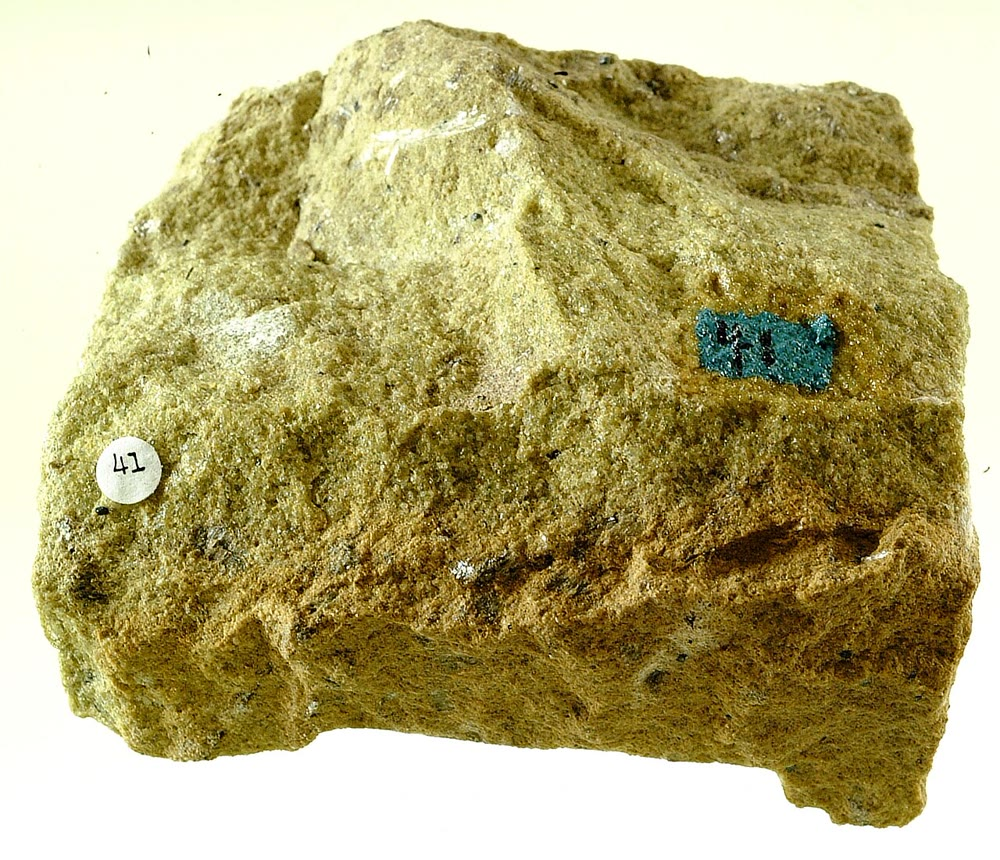
\includegraphics[width=\linewidth]{images/book4/b2-dunite.jpg}
\par\smallskip{\scriptsize دونيت، يكاد يكون كله أوليفين، فيه حبيبات سوداء صغيرة
من الكروميت؛ وعرض العيّنة \qty{8.5}{cm} \mbox{\textdir TLT (Mike Davis, CC0)}.}
\end{minipage}
\end{inthefield}
% ledger: casetta23:kimberlite, tulane:ocean-basins (Book 2), bgs:ultramafic

\section{التمارين}

\begin{exercise}[$\star$]\label{exo:b2:mantle-melting:1}
سمِّ كل صخر من نسب الأوليفين والأورثوبيروكسين والكلينوبيروكسين فيه
(في المئة): (أ) 93، 5، 2؛ (ب) 75، 25، 0؛ (ج) 60، 27، 13؛ (د) 30، 45، 25. (ه) أعطِ
اسم نموذج الوشاح العلوي (57 و28 و13 و\qty{2}{\percent} من السبينل) بعد
إعادة تطبيع سيليكاتاته الثلاثة إلى \qty{100}{\percent}.
\end{exercise}
% ledger: bgs:ultramafic, liang21:dmm-mode

\begin{exercise}[$\star$]\label{exo:b2:mantle-melting:2}
على مخطّط الديوبسيد--الأنورثيت، يبرد سائل فيه \qty{60}{\percent} من الأنورثيت.
(أ) عند أيّ درجة حرارة يبدأ بالتبلور، وأيّ معدن
يتكوّن؟ (ب) عند أيّ درجة حرارة يظهر المعدن الثاني، وما يكون عندئذ
تركيب السائل؟ (ج) ما تركيب أول سائل حين
يُسخَّن صخر فيه \qty{80}{\percent} من الديوبسيد و\qty{20}{\percent} من الأنورثيت،
وعند أيّ درجة حرارة يظهر؟
\end{exercise}
% ledger: bowen15:di-an

\begin{exercise}[$\star$]\label{exo:b2:mantle-melting:3}
(أ) احسب التدرّج الكظوم $\alpha T/(\rho c_p)$ بالكلفن لكل غيغاباسكال
من أجل $T_p = \qty{1350}{\celsius}$، $\alpha = \qty{4.0e-5}{K^{-1}}$، $\rho =
\qty{3300}{kg/m^3}$، $c_p = \qty{1000}{J/(kg.K)}$. (ب) كم كيلومترًا من
الوشاح تقابل غيغاباسكالًا واحدًا ($g = \qty{9.81}{m/s^2}$)؟ حوّل التدرّج إلى كلفن
لكل كيلومتر وقارنه بتدرّج حراري أرضي نموذجي قرب السطح،
نحو \qty{30}{K/km}.
\end{exercise}
% ledger: katz03:thermo, earle:settings (Book 2)

\begin{exercise}[$\star$]\label{exo:b2:mantle-melting:4}
(أ) احسب خط الصلابة الجاف للبيريدوتيت عند 0 و1 و2 و\qty{3}{GPa}. (ب) بكم
درجة يرتفع لكل غيغاباسكال قرب \qty{2}{GPa}؟ (ج) اشرح في جملة
واحدة لماذا يكون وشاح عند \qty{1400}{\celsius} وعند \qty{3}{GPa} صلبًا، بينما يكون
الوشاح نفسه إذا رُفع إلى \qty{2}{GPa} دون تبادل حرارة منصهرًا جزئيًا.
\end{exercise}
% ledger: katz03:solidus

\begin{exercise}[$\star\star$]\label{exo:b2:mantle-melting:5}
يبرد سائل فيه \qty{70}{\percent} من الديوبسيد و\qty{30}{\percent} من الأنورثيت.
(أ) قدّر درجة حرارة خط سيولته بالاستكمال الداخلي بين خط السيولة عند
\qty{20}{\percent} من الأنورثيت (\qty{1350}{\celsius}) وعند \qty{40}{\percent}
(\qty{1277.5}{\celsius}). (ب) أيّ معدن يتبلور أولًا؟ (ج) ما الكسر الكتلي
من النظام الذي تبلور حين يبلغ السائل الأوتكتيك؟
(د) ما نسبتا الديوبسيد والأنورثيت في الصخر النهائي؟
\end{exercise}
% ledger: bowen15:di-an

\begin{exercise}[$\star\star$]\label{exo:b2:mantle-melting:6}
(أ) احسب النسبة المئوية الكتلية لأكسيد \ce{SiO2} في الفورستريت \ce{Mg2SiO4} وفي
الإنستاتيت \ce{MgSiO3} ($M_{\ce{MgO}} = \qty{40.30}{g/mol}$، $M_{\ce{SiO2}} =
\qty{60.08}{g/mol}$). (ب) وجد بوين وأندرسن أن السائل البيريتكتيكي يتكوّن من
\qty{97.5}{\percent} من \ce{MgSiO3} و\qty{2.5}{\percent} من \ce{SiO2}: فما
محتواه من السيليكا؟ (ج) استعمل قاعدة الرافعة لحساب الكسر الكتلي للفورستريت
المتكوّن حين ينصهر الإنستاتيت عند \omterm{def:b2:mantle-melting:peritectic}{النقطة البيريتكتيكية}، وقارنه بقيمتهما
\qty{5.5}{\percent}. (د) ماذا يقتضي ذلك بشأن محتوى السيليكا في مصهور
\omterm{def:b2:mantle-melting:peridotites}{البيريدوتيت} مقارنةً بمحتواه في أورثوبيروكسينه؟
\end{exercise}
% ledger: bowen14:mgo-sio2

\begin{exercise}[$\star\star$]\label{exo:b2:mantle-melting:7}
باستعمال التدرّج الكظوم $T = T_p + 20P$ وخط الصلابة الجاف في النص، احسب
الضغط والعمق ($\qty{30.9}{km}$ لكل غيغاباسكال) اللذين يبدأ عندهما الانصهار
من أجل (أ) $T_p = \qty{1300}{\celsius}$ و(ب) $T_p = \qty{1450}{\celsius}$. (ج) بكم
كيلومترًا لكل \qty{10}{\celsius} يتعمّق البدء قرب
$T_p = \qty{1300}{\celsius}$؟ استعمل \cref{prop:b2:mantle-melting:onset}.
\end{exercise}
% ledger: katz03:solidus

\begin{exercise}[$\star\star$]\label{exo:b2:mantle-melting:8}
عند \qty{2.0}{GPa}، اعتبر أن \omterm{def:b2:mantle-melting:fraction}{كسر المصهور} يزداد خطيًا من خط الصلابة الجاف إلى
خط سيولة \omterm{def:b2:mantle-melting:peridotites}{اللرزوليت} $T_{\mathrm l} = 1475.0 + 80.0P - 3.2P^2$. من أجل $F = 0.10$:
(أ) احسب درجة حرارة الصخر المنصهر؛ (ب) احسب $(\partial
T/\partial P)_F$ و$(\partial T/\partial F)_P$؛ (ج) احسب الإنتاجية مع
$c_p = \qty{1000}{J/(kg.K)}$، $\alpha/\rho = \qty{1.21e-8}{m^3/(kg.K)}$
و$\Delta S = \qty{300}{J/(kg.K)}$. (د) كم تكون دون حرارة كامنة؟
\end{exercise}
% ledger: katz03:solidus, katz03:melting, katz03:thermo

\begin{exercise}[$\star\star$]\label{exo:b2:mantle-melting:9}
(أ) بكم يخفض 1 و5 و\qty{13}{\percent} من الماء المذاب في المصهور
خط الصلابة؟ (ب) ما خط الصلابة المشبع بالماء عند \qty{1}{GPa}؟ (ج) يحوي وشاحٌ
\qty{125}{ppm} من الماء كتلةً، ومعامل توزيع الماء بين
المعادن والمصهور 0.01. عند أول انصهار تمامًا، يحوي المصهور $X =
X_{\text{الكلي}}/D$: احسبه واحسب خفض خط الصلابة الذي يسبّبه.
\end{exercise}
% ledger: katz03:water

\begin{exercise}[$\star\star\star$]\label{exo:b2:mantle-melting:10}
(أ) في \cref{prop:b2:mantle-melting:triangle}، تحقّق من أن الوشاح الداخل إلى
قاعدة المثلث كل سنة يساوي الوشاح الخارج عبر ضلعيه. ولماذا
يجب أن يكون الضلعان مائلين بزاوية \ang{45} لوشاح يصعد بالسرعة $U$ ويغادر بالسرعة $U$؟
(ب) بيّن أنه، مع إنتاجية ثابتة $\Pi$ لكل غيغاباسكال، $h_c = \Pi\,\rho
g\,z_0^2/2$ (مع $P_0 = \rho g z_0$)، فتنمو القشرة مع مربع
عمق البدء. (ج) ظهرة تتباعد بمعدل كلي قدره \qty{50}{mm/yr}
وتصنع \qty{7.1}{km} من القشرة: ما حجم القشرة الذي يصنعه كل كيلومتر من الظهرة
في السنة، وما حجم الوشاح الذي تصهره إذا كان \omterm{def:b2:mantle-melting:fraction}{كسر المصهور} المتوسط
\qty{12}{\percent}؟
\end{exercise}

\begin{exercise}[$\star\star\star$]\label{exo:b2:mantle-melting:11}
في النظام الثلاثي في الشكل التخطيطي، للسائل $X$
\qty{60}{\percent} من A، و\qty{20}{\percent} من B و\qty{20}{\percent} من C؛
والأوتكتيك الثنائي $e_{AB}$ عند A 40، B 60 (في المئة)، \omterm{def:b2:mantle-melting:ternary}{والأوتكتيك الثلاثي} E عند
A 25، B 30، C 45. (أ) اكتب تركيب السائل حين يتبلور كسر كتلي $t$
من A النقي، وبيّن أن نسبة B إلى C تبقى 1. (ب) \omterm{def:b2:mantle-melting:ternary}{الخط
المتبلور المشترك} من $e_{AB}$ إلى E هو خط النقاط $e_{AB} + s(E - e_{AB})$: جِد
أين يلاقيه السائل، وكسر A المتبلور حتى ذلك الحين. (ج) حين
يبلغ السائل E، ما الكسر من النظام الذي لا يزال سائلًا؟ (لا يدخل C أيّ
بلّورة قبل E.) (د) كم من A وكم من B تبلور حتى ذلك الحين؟
\end{exercise}

\begin{exercise}[$\star\star\star$]\label{exo:b2:mantle-melting:12}
محتوى الماء في مصهور مشبع هو $X_{\mathrm{sat}} = 12P^{0.6} + P$
(في المئة، و$P$ بالغيغاباسكال). (أ) احسبه عند 1 و\qty{2}{GPa}، وخفض خط الصلابة
الذي يعطيه، وخط الصلابة المشبع بالماء عند الضغطين. (ب) لماذا لا يكاد
خط الصلابة المشبع يتغيّر بين 1 و\qty{2}{GPa} بينما يرتفع الجاف
بأكثر من \qty{100}{\celsius}؟ (ج) في إسفين وشاح عند \qty{2}{GPa}
و\qty{1100}{\celsius}، كم من الماء يجب أن يحوي المصهور لكي ينصهر الصخر؟
\end{exercise}
% ledger: katz03:water, katz03:solidus

\section{مسألة: تحت الظهرة}

\begin{problem}[{مسألة نهاية الأسبوع --- من التدرّج الكظوم للوشاح إلى سمك
القشرة المحيطية، ثم العودة إلى درجة حرارة الوشاح}]
\label{pb:b2:mantle-melting:1}
يصعد الوشاح تحت ظهرة على امتداد التدرّج الكظوم وينصهر. البيانات: التمدّد
الحراري $\alpha = \qty{4.0e-5}{K^{-1}}$؛ الكثافة $\rho = \qty{3300}{kg/m^3}$؛
السعة الحرارية النوعية $c_p = \qty{1000}{J/(kg.K)}$؛ إنتروبيا الانصهار $\Delta S =
\qty{300}{J/(kg.K)}$؛ $g = \qty{9.81}{m/s^2}$؛ خط الصلابة الجاف $T_{\mathrm s} =
1085.7 + 132.9P - 5.1P^2$ وخط سيولة \omterm{def:b2:mantle-melting:peridotites}{اللرزوليت} $T_{\mathrm l} = 1475.0 +
80.0P - 3.2P^2$ (\unit{\celsius}، و$P$ بوحدة \unit{GPa})؛ الإنتاجية المتوسطة
لنموذج الانصهار المضبوط، $\Pi = \qty{9}{\percent}$ لكل غيغاباسكال؛ معامل تفاعل
الكلينوبيروكسين قرب السطح 0.50؛ القشرة المرصودة \qty[uncertainty-mode=separate]{7.1 \pm 0.8}{km}
عند الظهرات العادية و\qty{20}{km} فوق لبّ عمود آيسلندا. اعتبر أن للوشاح
والقشرة الكثافة نفسها.

\noindent\textbf{الجزء الأول --- أين يبدأ الانصهار.}
\begin{enumerate}
\item حوّل $T_p = \qty{1350}{\celsius}$ إلى الكلفن.
\item احسب التدرّج الكظوم $\alpha T_p/(\rho c_p)$ بالكلفن لكل
غيغاباسكال، وقرّبه إلى أقرب عشرة.
\item كم كيلومترًا من الوشاح تقابل غيغاباسكالًا واحدًا؟ أعطِ التدرّج بالكلفن
لكل كيلومتر.
\item مع التدرّج الكظوم $T = 1350 + 20P$، اكتب المعادلة التربيعية لضغط البدء
$P_0$ وحلّها.
\item أعطِ العمق ودرجة الحرارة اللذين يبدأ عندهما الانصهار.
\item تحقّق من أن خط الصلابة عند $P_0$ يعطي درجة الحرارة نفسها.
\end{enumerate}

\noindent\textbf{الجزء الثاني --- كم من المصهور.}
\begin{enumerate}[resume]
\item عند \qty{1.5}{GPa}، احسب خط الصلابة وخط سيولة \omterm{def:b2:mantle-melting:peridotites}{اللرزوليت}
والفرق بينهما.
\item مع كسر مصهور يزداد خطيًا بينهما، أعطِ درجة حرارة
الصخر عند $F = 0.10$، بالدرجات المئوية وبالكلفن.
\item احسب $(\partial T/\partial P)_F$ و$(\partial T/\partial F)_P$ هناك.
\item احسب الإنتاجية في \cref{prop:b2:mantle-melting:productivity}، بالنسبة
المئوية لكل غيغاباسكال.
\item يعطي النموذج المضبوط $\Pi = \qty{9}{\percent}$ لكل غيغاباسكال في المتوسط.
لماذا هي أدنى؟ ومع $\Pi$، ما \omterm{def:b2:mantle-melting:fraction}{كسر المصهور} $F_{\max}$ الذي يُبلغ عند
السطح؟
\item يحوي الوشاح النموذجي \qty{13}{\percent} من الكلينوبيروكسين. عند أيّ كسر مصهور
يُستنفد قرب السطح؟ وهل البقايا تحت المحور
لرزوليت أم هارزبورجيت؟
\end{enumerate}

\noindent\textbf{الجزء الثالث --- القشرة.}
\begin{enumerate}[resume]
\item استعمل \cref{prop:b2:mantle-melting:triangle} مع $H = z_0$ لحساب
سمك القشرة.
\item ما \omterm{def:b2:mantle-melting:fraction}{كسر المصهور} المتوسط للمصهور المجمّع؟
\item قارن بالسمك المرصود.
\item يعطي النموذج الكامل في الشكل \qty{9.0}{km}. لماذا هو أرقّ من
تقديرك؟
\item بيّن أن $h_c = k P_0^2$ واحسب $k$ بالكيلومتر لكل غيغاباسكال
مربّع.
\end{enumerate}

\noindent\textbf{الجزء الرابع --- درجة حرارة الوشاح.}
\begin{enumerate}[resume]
\item احسب ضغط البدء $P_0$ الذي يصنع \qty{7.1}{km} من القشرة.
\item أعطِ العمق المقابل للبدء.
\item مع التدرّج الكظوم $T = T_p + 20P$، احسب درجة الحرارة الكامنة التي
تضع البدء عند ذلك الضغط.
\item أعد الحساب من أجل 6.3 و\qty{7.9}{km}: ما مدى $T_p$ الذي يسمح به
تشتّت القشرة؟
\item سمك القشرة \qty{20}{km} فوق لبّ عمود آيسلندا. احسب
درجة الحرارة الكامنة هناك، وزيادتها على درجة حرارة السؤال~20.
\item توحي حمم الجزر المحيطية بأعمدة أسخن بمقدار 200 إلى \qty{300}{\celsius} من
الوشاح المحيط. اقترح سببًا لكون القشرة تعطي زيادة أصغر.
\item بكم في المئة تثخن القشرة لوشاح أسخن بمقدار \qty{10}{\celsius}،
قرب الظهرة العادية؟
\item الظهرات البطيئة جدًا تصنع قشرة أرقّ. اشرح السبب بالمثلث.
\item اذكر \omterm{def:b2:mantle-melting:tp}{درجة الحرارة الكامنة للوشاح} تحت ظهرة عادية التي
يعطيها سمك القشرة، وهي الرقم الأساسي في هذه المسألة، وقارنها
بقيمة \qty{1350}{\celsius} من فيزياء المعادن وبالمدى من 1280 إلى
\qty{1400}{\celsius} من الحمم.
\end{enumerate}
\end{problem}
% ledger: katz03:solidus, katz03:melting, katz03:thermo, white:crust (Book 3), herzberg:tp (Book 3), katsura:adiabat (Book 3)
